\documentclass[12pt, a4paper]{article}
\usepackage{geometry}
\usepackage[utf8]{inputenc}
\usepackage{graphicx}
\usepackage{float}
\usepackage[most]{tcolorbox}
\usepackage[spanish,es-noshorthands]{babel}
\usepackage{titlesec}
\titleformat*{\section}{\large\bfseries}

\title{Sistemas Operativos \\\ Gestión de la Memoria}
\author{Acosta Quintana Lautaro Alejo}
\geometry {
    left=1.59cm,
    right=1.58cm,
    tmargin=1.9cm,
    bottom=2.534cm
}
\begin{document}
\maketitle
\tableofcontents
\break

El sistema operativo es el encargado de la tarea de subdivisión y a esta tarea se le denomina \textbf{gestión de la memoria}.
\section{Requisitos de la Gestión de la Memoria}
La gestión de la memoria debe satisfacer los siguientes requisitos:
\begin{itemize}
    \item Reubicación.
    \item Protección.
    \item Compartición.
    \item Organización Lógica.
    \item Organización Física.
\end{itemize}
\subsection{Reubicación}
Es necesario poder intercambiar procesos en la memoria principal para maximizar la utilización del procesador y si una vez que el programa se ha llevado al disco, solo pudiera ser colocado otra vez en la misma región donde estaba, esto sería contraproducente. Por lo que es necesario poder \textbf{reubicarlo} en un área de memoria diferente (esto posible gracias al intercambio o \textit{swap}).\\\\ 
\begin{figure}[H]
    \centering
    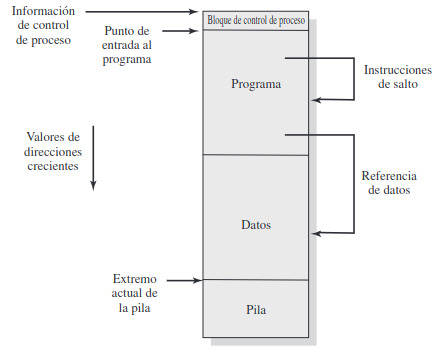
\includegraphics[width=10cm]{proceso1.jpeg}\par
    \caption{Requisitos de direccionamiento para un proceso}
\end{figure}
El sistema operativo necesita conocer la ubicación de la información de control del proceso y de la pila de ejecución, así como el punto de entrada que utiliza el proceso para iniciar la ejecución (Estas direcciones son fáciles de conseguir, ya que es el sistema operativo el encargado de traer el proceso a la memoria principal). Sin embargo, el hardware del procesador y el software del sistema operativo tendrán que ser capaces de traducir las referencias de memoria encontradas en el código del programa en direcciones de memoria físicas, que reflejen la ubicación actual del programa en la memoria principal.
\subsection{Protección}
Los programas de otros procesos no deben ser capcaes de referenciar sin permiso posiciones de memoria de un proceso, tanto en modo lectura como escritura. Todas las referencias de memoria generadas por un proceso deben comprobarse en tiempo de ejecución para poder asegurar ques e refieren sólo al pesacio de memoria asignado a dicho proceso. El procesador debe ser capaz de abortar tales instrucciones en el punto de ejecución.\\\\
Los requisitos de protección de memoria deben ser satisfechos por el procesador en lugar del sistema operativo, ya que el sistema operativo no podría anticiparse a todas las referencias que el programa hará e incluso, si fuera posible, sería muy costoso el cálculo para comprobarlos.

\begin{tcolorbox}[colback=cyan!10, colframe=blue!70, title=Nota]
    Sólo es posible evaluar la permisibilidad de una referencia (acceso a datos o salto) en tiempo de ejecución de la instrucción que realiza dicha referencia.
\end{tcolorbox}
\subsection{Compartición}
Cualquier mecanismo de protección debe permitir a varios procesos acceder a la misma porción de memoria principal. El sistema de gestión de memoria debe permitir el acceso controlado a áreas de memoria compartidas sin comprometer la protección esencial.
\subsection{Organización Lógica}
La memoria principal de un computador se organiza como un espacio de alamcenamiento lineal o unidimensional, compuesto por una secuencia de bytes o palabras. A nivel físico, la memoria secundaria está organizada de forma similar. En cambio, la mayoría de los programas se organizan en módulos (que pueden ser modificables o no).\\\\ 
Si el sistema operativo y el hardware del computador pueden tratar de forma efectiva los programas de usuarios y los datos en la forma de módulos, se logran las siguientes ventajas:
\begin{enumerate}
    \item Los módulos se pueden escribirt y compilñar independientemente, con todas las referencias de un módulo desde otro resueltas por el sistema en tiempo de ejecución.
    \item Con una sobrecarga adicional, se puede proporcionar grados de protección a los módulos (sólo lectura, sólo ejecución).
    \item Es posible introducir mecansimos por los cuales los módulos se pueden compartir entre los procesos. La ventaja de esto es que corresponde con la forma en la que el usuario ve el problema, por lo que es más facil para el especificar la compartición deseada.
\end{enumerate}
\begin{tcolorbox}[colback=cyan!10, colframe=blue!70, title=Nota]
    La herramienta más adecuada para estos requisitos es la \textbf{segmentación}.
\end{tcolorbox}

\subsection{Organización Física}
La organización del flujo de información entre la memoria principal y secundaria supone una de las preocupaciones principales del sistema. la responsabilidad para este flujo podría asignarse a cada programar, pero no es deseable o incluso practicable por dos motivos:
\begin{enumerate}
     \item La memoria principal disponible para un programas podría ser insuficiente. En este caso tendría que usarse \textbf{\textit{overlaying}} (\textbf{superposición}) en la cual los programas y sus datos se organizando de manera que pueda asignarse la misma región de memoria a varios módulos, con un programa principal responsables de intercambiar los módulos entre disco y memoria. La programación con \textit{overlay} malgasta tiempo del programador.
     \item En un entorno multiprogramado, el programador no conoce ne tiempo de codificacińo cuánto espacio estará disponible o dónde se localizara dihco espacio.
\end{enumerate}
La tarea de mover al información entre los dos niveles de memoria debería ser una responsabilidad del sistema.

\section{Particionamiento de la Memoria}
La operacioón principal de la gestión de la memoria es traer los procesos a la memoria principal para que el procesador los pueda ejectuar. Una de estas técnicas es el particionamiento.
\subsection{Particionamiento Fijo}
El esquema más simple para gestionar la memoria disponible es repartir en regiones con límites fijos.
\subsubsection{Tamaños de partición}
\begin{figure}[H]
    \centering
    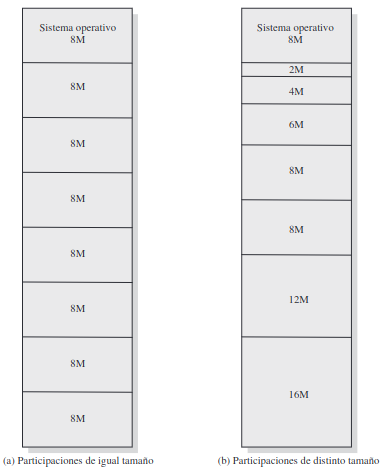
\includegraphics[width=10cm]{particionfija.png}\par
    \caption{Ejemplo de particionamiento fijo en una memoria de 64MB}
\end{figure}
Existen dos alternativas para el particionamiento fijo. Una consiste en hacer uso de particiones del mismo tamaño; en este caso cualquier procesos con tamaño menor o igual puede cargarse en la partición disponible. Si todas las particiones están llenas y no hay ningún proceso en estado Listo o Ejecutando, el sistema puede mandar a \textit{swap} a un proceso de cualquier partición y cargar otro. Existen dos dificultades con esta estrategía:
\begin{itemize}
    \item Un programa puede ser demasiado grande para entrar en una partición. En este caso el programador debe diseñar el programa con uso de \textit{overlays}. cuando se necesita un módulo que no está presente, el programa de usuario debe cargar dicho módulo en la partición del programa superponéndolo (\textit{overlaying}) a cualquier programa o dato que haya allí.
    \item La utilización de la memoria principal es extremadamente ineficiente. Este fenómeno, en el cual hay espacio interno malgastado debido al hecho de que el bloque de datos cargado es menor que la partición, se conoce como \textbf{framentación interna}.
\end{itemize}
Ambos problemas se pueden mejorar pero no resolver, utilizando particiones de tamaño diferente.
\subsubsection{Algoritmo de ubicación}
\begin{figure}[H]
    \centering
    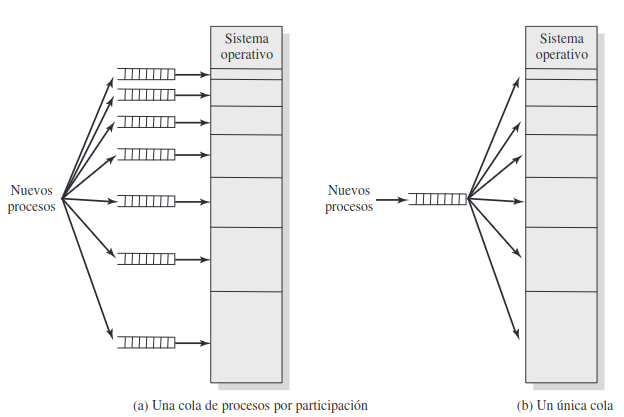
\includegraphics[width=12cm]{particionfija2.png}\par
    \caption{Asignación de memoria para particionamiento fijo.}
\end{figure}
Con particiones del mismo tamaño, la ubicación de los procesos en memoria es trivial.\\\\ 
Con particiones de diferente tamaños, hay dos formas de asignar los procesos a las particiones. \\ 
\begin{itemize}
    \item Asignar cada proceso a la partición más pequeña dentro de la que cabe. En este caso se utiliza una cola de planificación para cada partición, que mantenga procesos en disco destinados a dicha partición. La ventaja de esta técnica es que se minimiza la \textbf{fragmentación interna}, aunque no es óptima para un sistema complejo. Se asume que se conoce el tamaño máximo de memoria que un proceso requerirá, en caso contrario, la única alternativa es un esquema de \textit{overlays} o usar memoria virtual. Es la técnica más sencilla.
    \item Emplear una única cola para todos los procesos. En el momento de cargar un proceso en la memoria principal, se selecciona la partición más pequeña disponible capaz de albergar a dicho proceso.
\end{itemize}
Si todas las particiones están ocupadas, se debe llevar a cabo una decisión para enviar a \textit{swap} a algún proceso.
\begin{tcolorbox}[colback=cyan!10, colframe=blue!70, title=Nota]
    Tiene preferencia a la hora de ser expulsado a disco el proceso que ocupe la partición más pequeña que pueda albergar al proceso entrante.
\end{tcolorbox}
\subsection{Particionamiento Dinámico}
Con particionamiento dinámico, las particiones son de longitud y número variable. Cuando se lleva un proceso a la memoria principal, se le asigna exactamente tanta memoria como requiera.
\begin{figure}[H]
    \centering
    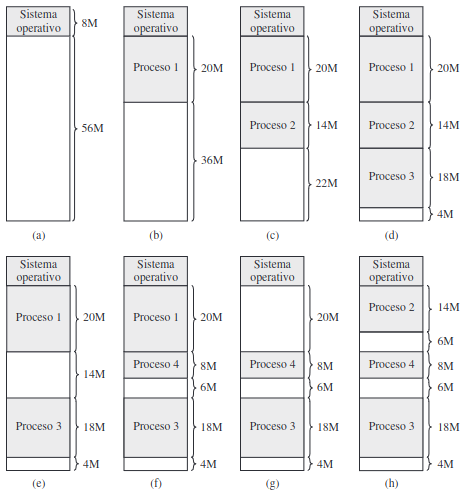
\includegraphics[width=12cm]{particiondinamica.png}\par
    \caption{El efecto del particionamiento dinámico.}
\end{figure}
Como se observa en la Figura 4., el método comienza correctamente pero lleva a una situación en la cual existen muchos huevos pequeños en la memoria. A medida que pasa el tiempo, la memoria se fragmenta cada vez más y la utilización decrementa. Este fenómeno se conoce como \textbf{fragmentación externa}, indicando que la memoria que es externa a todas las particiones se fragmenta de forma incremental.\\\\ 
Una técnica para elimar la fragmentación externa es la \textbf{compactación}: de vez en cuando, el sistema operativo desplaza los procesos en memoria, de forma que se encuentren contiguos y de este modo toda la memoria libre se encontrará unida en un bloque. La desventaja de la compactación es que se trata de un procedimiento que consume tiempo y recursos del procesador.
\begin{tcolorbox}[colback=cyan!10, colframe=blue!70, title=Nota]
    La compactación requiere la capacidad de \textbf{reubicación dinámica} (mover un programa desde una región a otra en la memoria principal sin invalidar las referencias de memoria de cada programa).
\end{tcolorbox}
\subsubsection{Algoritmo de ubicación}
Tres algoritmos de colocación que pueden considerarse son \textit{best-fit}, \textit{first-fit}, \textit{next-fit} y \textit{worst-fit}; todos limitas a elegir entre los bloques libre de la memoria principal que son iguales o más grandes que el proceso que va a llevara  la memoria. 
\begin{itemize}
    \item \textbf{Best-fit} elige el bloque más cercano en tamaño a la petición.
    \item \textbf{First-fit} comienza a analizar la memoria desde el principio y escoge el primer bloque disponible que sea suficientemente grande.
    \item \textbf{Next-fit} comienza a analizar la memoria desde la última colocación y elige el siguinete bloque disponible que sea suficientemente grande.
    \item \textbf{Worst-fit} elige el mayor bloque de memoria libre para un proceso.
\end{itemize}
\begin{tcolorbox}[colback=cyan!10, colframe=blue!70, title=Nota]
    Cual técnica es mejor depende de la secuencia exacta de intercambio y tamaño de los procesos. Algunos comentarios son:
    \begin{itemize}
        \item First-fit es el más sencillo y normalmente es el mejor y más rápido.
        \item Next-fit tiende a producir resultados ligeramentes peores que First-fit.
        \item Next-fit lleva más frecuentemenete a una asignación de un bloque libre al final de la memoria el cual normalmente es el bloque más grande de memoria libre, lo que lleva a que se divida en pequeños fragmentos y requiera más frecuentemente la compactación.
        \item First-fit puede dejar el final del espacio de almacenamiento con pequeñas particiones libres que necesitan buscarse en cada paso del primer ajuste siguiente.
        \item Best-fit tiene normalmente el peor comportamiento, debido a que busca el bloque más pequeño que satisfaga la petición garantiza que el fragmento que quede sea lo más pequeño posible. Por esto la compactación debe realizarse con mayor frecuencia que en el resto de algoritmos.
    \end{itemize}
\end{tcolorbox}
\subsubsection{Algoritmo de reemplazamiento}
En un sistema multiprogramado, puede ocurrir que todos los procesos de la memoria principal estén en estado bloqueado y no haya suficiente memoria para un proceso adicional, incluso después de una compactación. Para evitar malgastar tiempo del procesador, el sistema operativo intercambiará alguno de los procesos entre la memoria principal y disco para hacer sitio a un nuevo proceso o para un proceso que se encuentre en estado Listo-Suspendido.
\subsection{Sistema Buddy}
Como se ha visto, un esquema de particionamiento fijo limita el número de procesos activos y utiliza el espacio ineficientemente si existe un mal ajuste entre el tamaño de las particiones y los procesos. Un esquema de particionamiento dinámico es más complejo de mantener e incluye la sobrecarga de la compactación. \\ 
Por lo tanto, un compromiso interesante es el sistema \textit{buddy}. En donde los bloques de memoria disponibles son de tamaño $2^k$, $L \leq K \leq U$, donde
\begin{itemize}
    \item $2^L$ = bloque de tamñao más pequeño asignado.
    \item $2^U$ = bloque de tamaño mayor asignado; normalmente $2^U$ es el tamaño de la memoria completa disponible
\end{itemize}
El espacio completo disponible se trata como un único bloque de tamaño $2^U$. Si se realiza una petición de tamaño $s$, tal que $2^{U-1}\le s \leq 2^U$, se asigna el bloque entero. En otro caso, el bloque se divide en dos bloques \textit{buddy} iguales de tamaño $2^{U-1}$. Si $2^{U-2}\le s \leq 2^{U-1}$, entonces se asigna la petición a uno de los otros dos bloques. En otro caso, uno de ellos se divide por la mitad de nuevo. Este proceso continúa hasta que el bloque más pequeño mayor o igual a $s$ es generado y se asigna a la petición. En cualquier momento el sistema \textit{buddy} mantiene una lista de huecos de cada tamaño $2^i$. Un hueco puede eliminarse de la lista ($i+1$) dividiéndolo por la mitad para crear dos bloques de tamaño $2^i$ en la lista $i$. Siempre que un par de bloques de la lista $i$ no se encuentren asignados, son eliminados de dicha lista y unidos en un único bloque de la lista ($i+1$). Si se lleva a cabo una petición de asignación de tamaño $k$ tal que $2^{i-1}\le k \leq 2^i$, se utiliza el siguiente algoritmo recursivo para encontrar un huevo de tamaño $2^i$:
\begin{verbatim}
    void obtener_huevo(int i) {
        if (i==(U+1))
            <fallo>;
        if (<lista_i vacía>) {
            obtener_huevo(i+1);
            <dividr huevo en dos buddies>;
            <colocar buddies en lista_i>;
        }
        <tomar primer huevo de la lista_i;
    }
\end{verbatim}

El sistema \textit{buddy} es un compromiso razonable para eliminar las desventajas de ambos esqeumas de particionamiento, fijo y variable. El sistema se ha utilizado en sistemas paralelos como forma eficiente de asignar y liberar programas paralelos.
\begin{figure}[H]
    \centering
    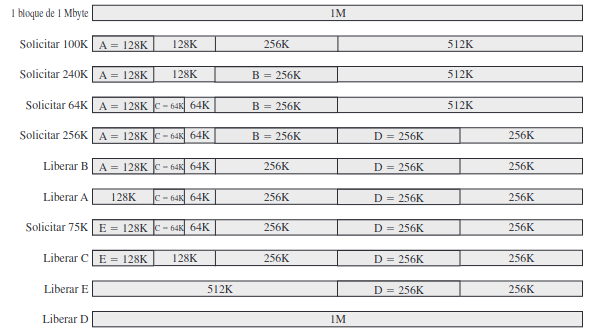
\includegraphics[width=15cm]{buddy.png}\par
    \caption{Ejemplo de sistema \textit{buddy}.}
\end{figure}

\subsection{Reubicación}
Cuando se utiliza el esquema de particionamiento fijo (Figura 3.a), se espera que un proceso siempre se asigne a la misma partición. Cuando el proceso se carga por primera vez, todas las referencias de la memoria relativas del código se reemplazxan por direcciones de la memoria principal absolutas, determinadas por la dirección bas edel proceso cargado.\\\\ 
En el caso de particiones de igual tamaño (Figura 2) y en el caso de una única cola de procesos para particiones de distinto tamaño (Figura 3.b), un proceso puede ocupar diferentes particiones durante su ciclo de vida. Por lo tanto, las ubicaciones (de instrucciones y datos) referenciadas por un proceso no son fijas. Para resolver este problema, se realiza una distinción entre tipós de direcciones. Una \textbf{dirección lógica} es una referencia a una ubicación de memoria independiente de la asignación actual de datos a la memoria; se debe llevar a cabo una traducción a una dirección física antes de alcanzar el acceso a la memoria. Una \textbf{dirección relativa} es un ejemplo particular de dirección lógica, en la que es expresada como una ubicación relativa a algún punto conocido, normalmente un valor en un registro del procesador. Una \textbf{dirección física}, o dirección absoluta es una ubicación real de la memoria principal. \\\\ 
Los programas que emplean direcciones relativas de memoria se cargan utilizando carga dinámica en tiempo de ejecución. Normalmente, todas las referencias de memoria de los procesos cargados son relativas al origen del programa. Por tanto, se necesita un mecanismo de hardware para traducir las direcciones relativas a direcciones físicas de la memoria principal, en tiempo de ejecución de la instrucción que contiene a dicha referencia. \\\\ 
Cuando un proceso se asigna al estado ejecutando, un registro especial del procesador, llamado registro base, carga la dirección inicial del programa en la memoria principal. Existe un registro \textbf{valla} que indica el final de la ubicación del programa; estos valores se establecen cuando el programa se carga en la memoria cuando la imagen del proceso se lleva a la memoria. A lo largo de la ejecución del proceso, se encuentran direcciones relativas. Éstas incluyen los contenidos del registro de las instrucciones, las direcciones de intrucciones que ocurren en los saltos e instrucciones \textit{call}, y direcciones de datos existentes en instrucciones de carga y almacenamiento. El procesador manipula cada dirección relativa, a través de dos pasos. Primero, el valor del registro base se suma a la dirección relativa para producir una dirección absoluta. Segundo, la dirección resultante se compara con el valor del registro \textbf{valla}. Si la dirección se encuentra dentro de los límites, entonces se puede llevar a cabo la ejecución de la instrucción. En otro caso, se genera una interrupción, que debe manejar el sistema operativo de algún modo. \\\\ 
El esquema de la Figura 6 permite que se traigan a memoria los programas y que se lleven a disco, a lo largo de la ejecución. También proporcionan una medida de protección: cada imagen del proceso está asilada mediante los contenidos de los registros base y valla. Además, evita accesos no autorizados por parte de otros procesos.
\begin{figure}[H]
    \centering
    \includegraphics[width=15cm]{reubicación.png}
    \caption{Sosporte hardware para la reubicación.}
\end{figure}











\section {Bibliografía}
\begin{itemize}
    \item Stallings, W. (2005). Sistemas operativos. Aspectos internos y principios de diseño (Quinta ed.). Pearson Education.
\end{itemize}
\end{document}
